% heatmap regression works
% limited by heatmap resolution
% adapt heatmap with upsampling (unet \cite{ronneberger2015unetconvolutionalnetworksbiomedical})?
% different approach -> forgoes heatmap limiation
% easily adapted to crude parameter estimation (important for low-latency searches), but this wont be covered here

The previous chapter showed that heatmap regression performs well for GW searches. However, the approach is limited by the time resolution of the output heatmap, which becomes problematic for close overlaps. 
One possible solution would be to increase the heatmap resolution, for example by adding \emph{upsampling} steps after the transformer encoder, similar to U-Net architectures \cite{ronneberger2015unetconvolutionalnetworksbiomedical}. 

In this chapter, a different approach is investigated, forgoing the heatmap approach entirely. Instead, a fully end-to-end model is developed: for a given sample, the model directly outputs multiple GW candidates, each with a signal score and time location. 
The approach is based on the Detection Transformer (DETR) \cite{10.1007/978-3-030-58452-8_13}, which was originally developed for object detection in images and is modified here to handle time series instead.
Although not implemented in this thesis, such a model can simply be adapted to return an estimate of the signal parameters as well, which is important for low-latency searches.

\section{Architecture}

\begin{figure}
	\centering
	\makebox[\textwidth]{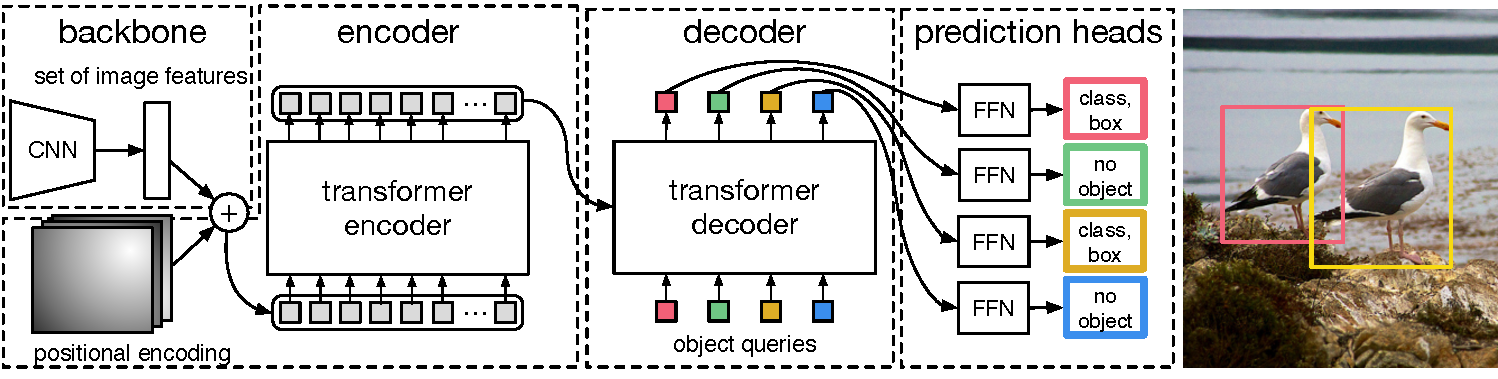
\includegraphics[width=16cm]{multiple_signal_detection/images/DETR_detail_seagulls}}
	\caption{Original DETR~\cite{10.1007/978-3-030-58452-8_13} architecture for image object detection. The model outputs multiple object class scores and bounding boxes.}
	\label{fig:detr:detr}
\end{figure}

\begin{figure}
	\centering
	\makebox[\textwidth]{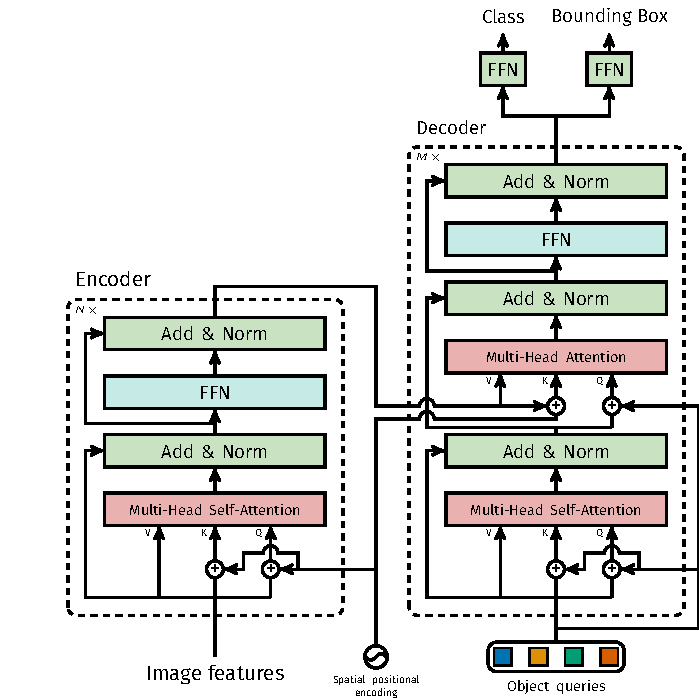
\includegraphics[width=11cm]{multiple_signal_detection/images/transformer}}
	\caption{Detailed implementation of the transformer used in DETR~\cite{10.1007/978-3-030-58452-8_13}. Positional encodings are not applied before the value projections.}
	\label{fig:detr:transformer}
\end{figure}

% explain architecture roughly see fig
% similar to transformer-encoder heatmap regressor
% instead of cls head transformer decoder (has been shown to improve performance)
% each query is read out via a cls and pos head + other parameters heads?

The DETR architecture consists of a CNN backbone, a transformer encoder, and a transformer decoder. Up to the encoder, the architecture is similar to the transformer-based heatmap-regressor. The difference is that the encoder output tokens are not read out directly to produce a heatmap, but serve as the source sequence of a transformer decoder. 
The decoder takes a number of learned \emph{queries} as its target sequence. The decoder output is read out with two prediction heads to produce a class score and the signal coalescence time. In principle, by appending more prediction heads, this architecture can be adapted to return other parameters as well.
See a schematic of the original architecture in Fig.~\ref{fig:detr:detr}. In a way, DETR is a natural extension of the ViT~\cite{DBLP:journals/corr/abs-2010-11929} architecture to multiple classification tokens.

One limitation of the DETR architecture is that the number of possible predictions per sample is fixed by the query count. This problem can be dealt with by simply choosing the number of queries to be sufficiently high. 

% details
% same CNN -> 512 tokens, 256 dim -> 64 embed dim
% transformer: 6 layers 8 heads
% encoder: sinusoidal, decoder: learned, only applied before q,k projections see fig
% decoder: 16 queries (refer to event rate)
% ff_dim = 1024, dropout = 0.1
% class head, time head
% \SI{6.2}{\mega\nothing} parameters, \SI{7}{\giga\byte}

For the CNN backbone, the same ResNet model as previously is employed. Given samples with a length of \SI{64}{\second}, the backbone outputs $512$ vectors of size $256$. A convolution operation with kernel size one projects these onto the embedding dimension $d_\text{embed}=64$. Both the transformer encoder and the decoder consist of six layers and eight heads, and employ FFNs with hidden dimension $d_\text{ff}=1024$. A dropout probability of \SI{10}{\percent} is used throughout the model. The transformer employs sinusoidal encodings for the encoder tokens and learned positional embeddings for the queries. Following the original architecture, these are applied before the query and key projections only (see Fig.~\ref{fig:detr:transformer}).

A total of $16$ queries is chosen. For the higher event-rate estimate of $\lambda=\SI{E+6}{\per\year}$, the probability for more than $16$ signals in a $T=\SI{64}{\second}$ long sample is negligible:
\begin{equation}
	P(n>16) = 1-\sum_{k=0}^{16}\,\frac{(\lambda T)^k}{k!}\,\e^{-\lambda T} = \SI{7E-9}{\percent},
\end{equation}
making this choice more than sufficient. These queries are learnable parameters of size $d_\text{embed}$, which are initialized as zero. After being passed through the decoder, each query is read out via two prediction heads.
The class score is obtained through,
\begin{equation}
\begin{aligned}
	n &= \mathrm{LayerNorm}(x),\\
	h &= \mathrm{ReLU}(\mathrm{Linear}_{64\rightarrow1024}(n)),\\
	z_c &=\mathrm{Linear}_{1024\rightarrow1}(h),
\end{aligned}
\end{equation}
which is later passed through a sigmoid layer. For the time prediction, the prediction head reads,
\begin{equation}
\begin{aligned}
	n &= \text{LayerNorm}(x),\\
	h_1 &= \text{ReLU}(\text{Linear}_{64\rightarrow1024}(n)),\\
	h_2 &= \text{ReLU}(\text{Linear}_{1024\rightarrow1024}(h_1)),\\
	h_3 &= \text{ReLU}(\text{Linear}_{1024\rightarrow1024}(h_2)),\\
	z_t &= \text{Linear}_{1024\rightarrow1}(h_3).
\end{aligned}
\end{equation}
This value is also passed through a sigmoid layer to normalize the prediction to $[0,1]$ in units of sample duration. In total, the network has \SI{6.2}{\mega\nothing} trainable parameters.

\section{Training}

\begin{figure}
	\centering
	\begin{minipage}{\textwidth}
	\centering
	\makebox[\textwidth]{
	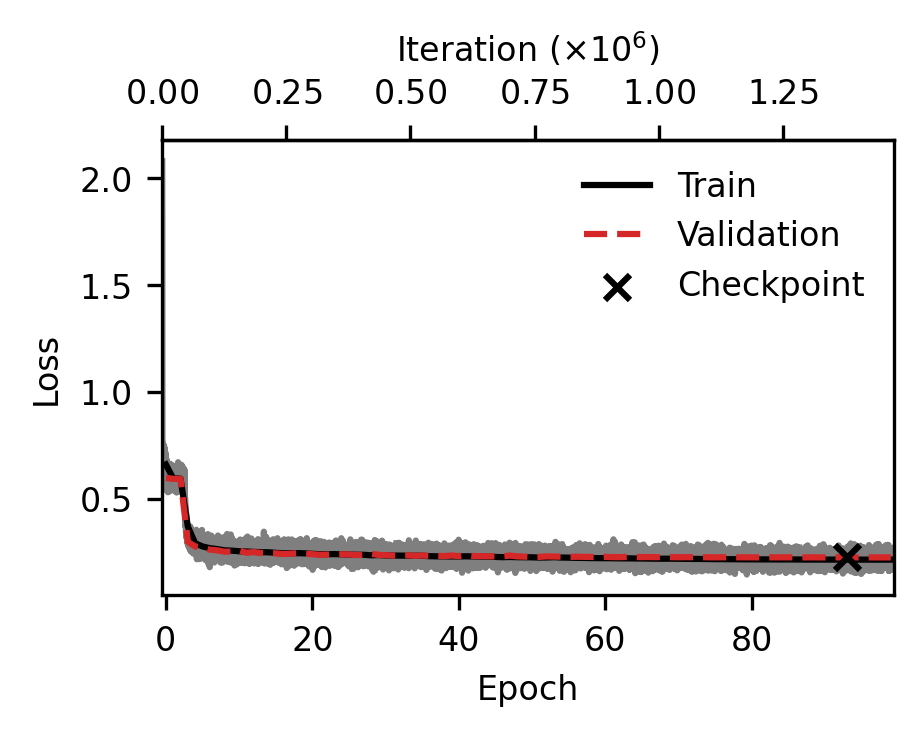
\includegraphics[width=8cm]{multiple_signal_detection/plots/learning_curves/detr_loss}
	}
	\caption{DETR learning curve. Total loss computed over the training dataset after each step (\emph{grey}) and averaged over each epoch (\emph{black}). Validation dataset loss (\emph{red}). The minimum validation-loss checkpoint is indicated.}
	\label{fig:detr:learning_curve}
	\end{minipage}
	\begin{minipage}{\textwidth}
	\centering
	\makebox[\textwidth]{
	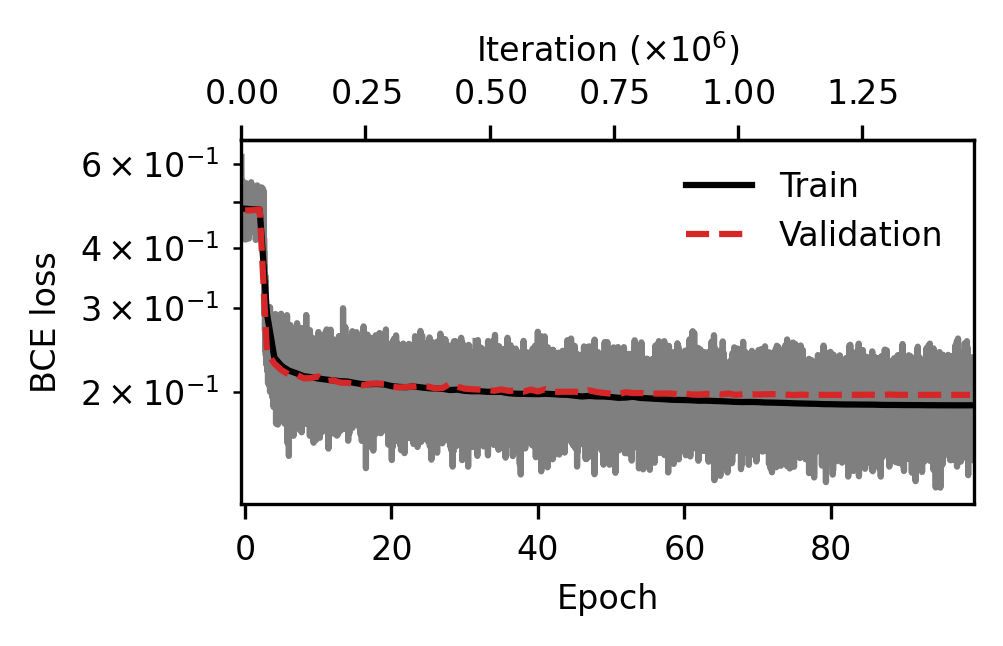
\includegraphics[width=8cm]{multiple_signal_detection/plots/learning_curves/detr_bce_loss}
	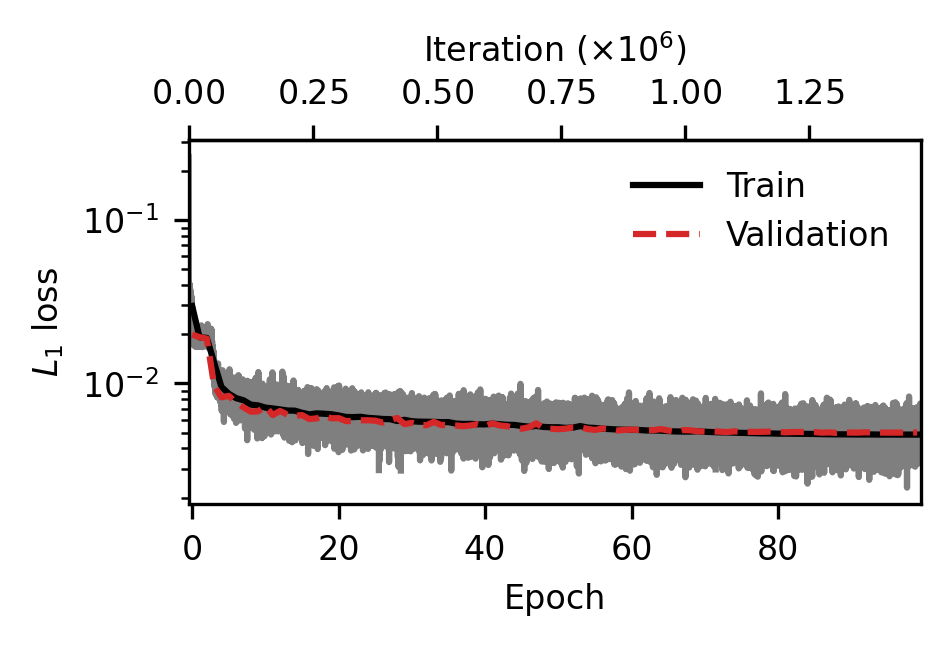
\includegraphics[width=8cm]{multiple_signal_detection/plots/learning_curves/detr_l1_loss}
	}
	\caption{Evolution of both loss terms during training. BCE loss (\emph{left}) and time prediction $L_1$ loss (\emph{right}).}
	\label{fig:detr:tandem}
	\end{minipage}
\end{figure}

%\begin{figure}
%	\centering
%	\makebox[\textwidth]{
%		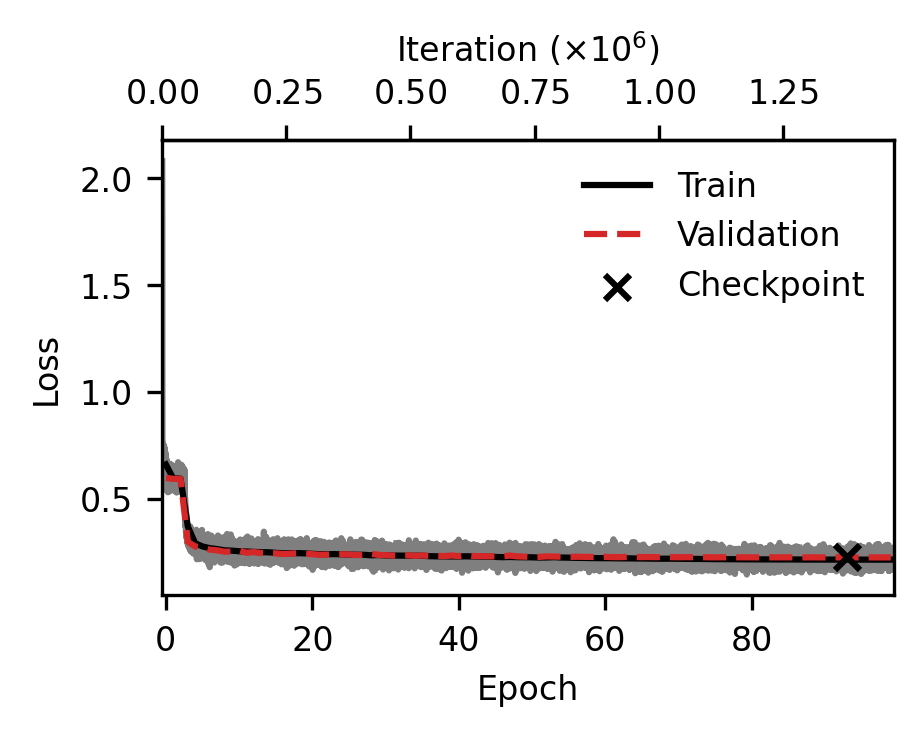
\includegraphics[width=8cm]{multiple_signal_detection/plots/learning_curves/detr_loss}
%	}
%	\caption{DETR learning curve. Total loss computed over the training dataset after each step (\emph{grey}) and averaged over each epoch (\emph{black}). Validation dataset loss (\emph{red}). The minimum validation-loss checkpoint is indicated.}
%	\label{fig:detr:learning_curve}
%\end{figure}
%\begin{figure}
%	\centering
%	\makebox[\textwidth]{
%		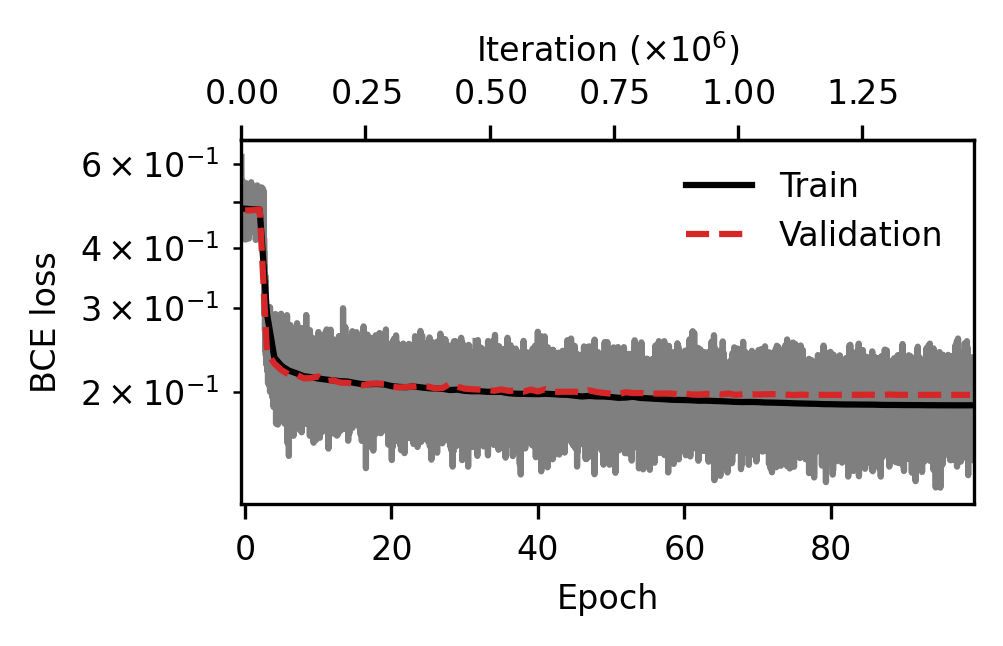
\includegraphics[width=8cm]{multiple_signal_detection/plots/learning_curves/detr_bce_loss}
%		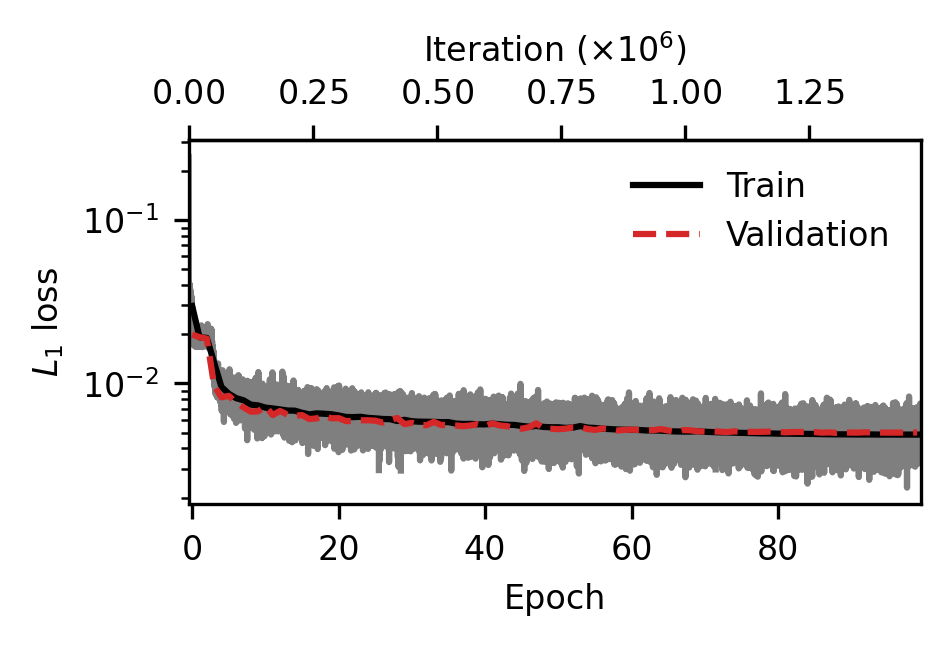
\includegraphics[width=8cm]{multiple_signal_detection/plots/learning_curves/detr_l1_loss}
%	}
%	\caption{Evolution of both loss terms during training. BCE loss (\emph{left}) and time prediction $L_1$ loss (\emph{right}).}
%	\label{fig:detr:tandem}
%\end{figure}

% loss function: train class and position in tandem 
% if c=0 time prediction is zeroed out
% what is the ground truth y?
% match m signals to m<n preds
% for unmatched preds the corresponding ground-truth is noise

For any given sample, the DETR architecture implemented here produces $m=16$ predictions $\hat{y}=\{(\hat{c}_j,\hat{t}_j)\}_{j=1}^{m}$, each comprising a signal score and coalescence time. The network is of course free to output predictions with $\hat{c}=0$, \emph{i.e.}\ noise predictions, which are discarded after thresholding. The class score and time prediction are trained in tandem, employing a BCE loss and an $L_1$ loss, summed over all predictions:
\begin{equation}
	\pazocal{L}(y, \hat{y}) = \sum_{j=1}^m \pazocal{L}_\text{BCE}(c_j, \hat{c}_j) + c_j\,\lambda|t_j - \hat{t}_j|.
\end{equation}
For predictions where the ground-truth class is noise, $c=0$, the time prediction loss is simply zeroed out. Since for random predictions the average BCE loss is $\pazocal{L}_\text{BCE}=\ln 2\approx0.69$, while the  $L_1$ loss to the nearest signal is only of order \SI{E-2}{}, the $L_1$ term is up-weighted by a factor $\lambda=6$. The exact value is chosen empirically.
The architecture makes use of \emph{auxiliary} losses, where the loss is computed over the output at each of the six decoder layers.

% how do we match? -> hungarian
% minimize total matching cost
% from this we get assignment function pi
% inverse gives indices i of signals matched to predictions j

Up to this point, it has been quietly swept under the rug what the ground truth $y=\{(c_j, t'_j)\}_{j=1}^{m}$ corresponding to the $m$ predictions actually looks like. 
For this purpose, all signals $\{t_i\}_{i=1}^{n}$ (where $n<m$) are assigned to predictions by a matching algorithm. Then the ground truth is constructed with
\begin{equation}
	\label{eq:detr:ground_truth}
	y_j = (c_j, t'_j) = \begin{cases}
		(1, t_i) & \text{if signal $i$ is matched to prediction $j$,} \\
		(0, \varnothing) & \text{else.}
	\end{cases}
\end{equation}
For unmatched predictions, the ground-truth coalescence time does not matter as the corresponding $L_1$ loss is zeroed out anyway.

Following \cite{10.1007/978-3-030-58452-8_13}, signals $i$ and predictions $j$ are matched by minimizing the cost,
\begin{equation}
	\pazocal{L}_\text{cost}(t_i, \hat{y}_j) = -\hat{c}_j + \lambda|t_i-\hat{t}_j|,
\end{equation}
where again $\lambda=6$.
Let $\tau:\pazocal{I}\rightarrow\pazocal{J}'$ denote an \emph{assignment function} mapping the signal indices $\pazocal{I} = \{1, 2, \dots, n\}$ to the subset of matched prediction indices $\pazocal{J}' \subset\pazocal{J} = \{1, 2, \dots, m\}$. The \emph{optimal} assignment function $\pi$ will be the realization of $\tau$ that minimizes the total assignment cost over all signals $i$ and corresponding predictions $\tau(i)$:
\begin{equation}
	\pi = \argmin_\tau \sum_{i=1}^n \pazocal{L}_\text{cost}(t_i, \hat{y}_{\tau(i)}).
\end{equation}
This is referred to as an \emph{assignment problem} and can be solved with methods implemented by SciPy \cite{2020SciPy-NMeth}. 

It can be seen that the index $i$ of a signal that is matched to a prediction $j$ is given by $\pi^{-1}(j)$. This function $\pi^{-1}(j)$ is only defined for those predictions $j$, which have been matched, $j\in\pazocal{J}'$. Thus with Eq.~\ref{eq:detr:ground_truth}, the ground truth $y_j$ that corresponds to $\hat{y}_j$ can be constructed as,
\begin{equation}
	y_j = \begin{cases}
		(1, t_{\pi^{-1}(j)}) & \text{if $j\in\pazocal{J}'$,} \\
		(0, \varnothing) & \text{else.}
	\end{cases}
\end{equation}
To differentiate this scheme from greedy matching, which is used for evaluation, the matching algorithm here will be referred to as \emph{Hungarian matching} following the terminology in \cite{10.1007/978-3-030-58452-8_13}.

% adamw with lr e-4, lam e-4, for a maximum of 100 epochs
% vram = 7gib, check maybe?
% cosine annealing with 5000 steps warmup

The DETR model is trained on the same \SI{1}{\mega\nothing} sample dataset as the heatmap models. The AdamW optimizer is used with a learning rate of \SI{E-4}{}, a weight decay of \SI{E-4}{} and a batch size of $64$. Training is performed for a maximum of $100$ epochs. For this, a cosine-annealing learning-rate schedule is employed with a warmup of $5000$ steps. 

See the total loss learning curve in Fig.~\ref{fig:detr:learning_curve}. The validation loss reaches its minimum after $93$ epochs. This checkpoint is used for all following results. Fig.~\ref{fig:detr:tandem} shows the evolution of the individual loss terms. It can be seen that both the class score and the time prediction have been successfully optimized in tandem. 

\section{Comparison with Heatmap Regression}

\begin{figure}
	\centering
	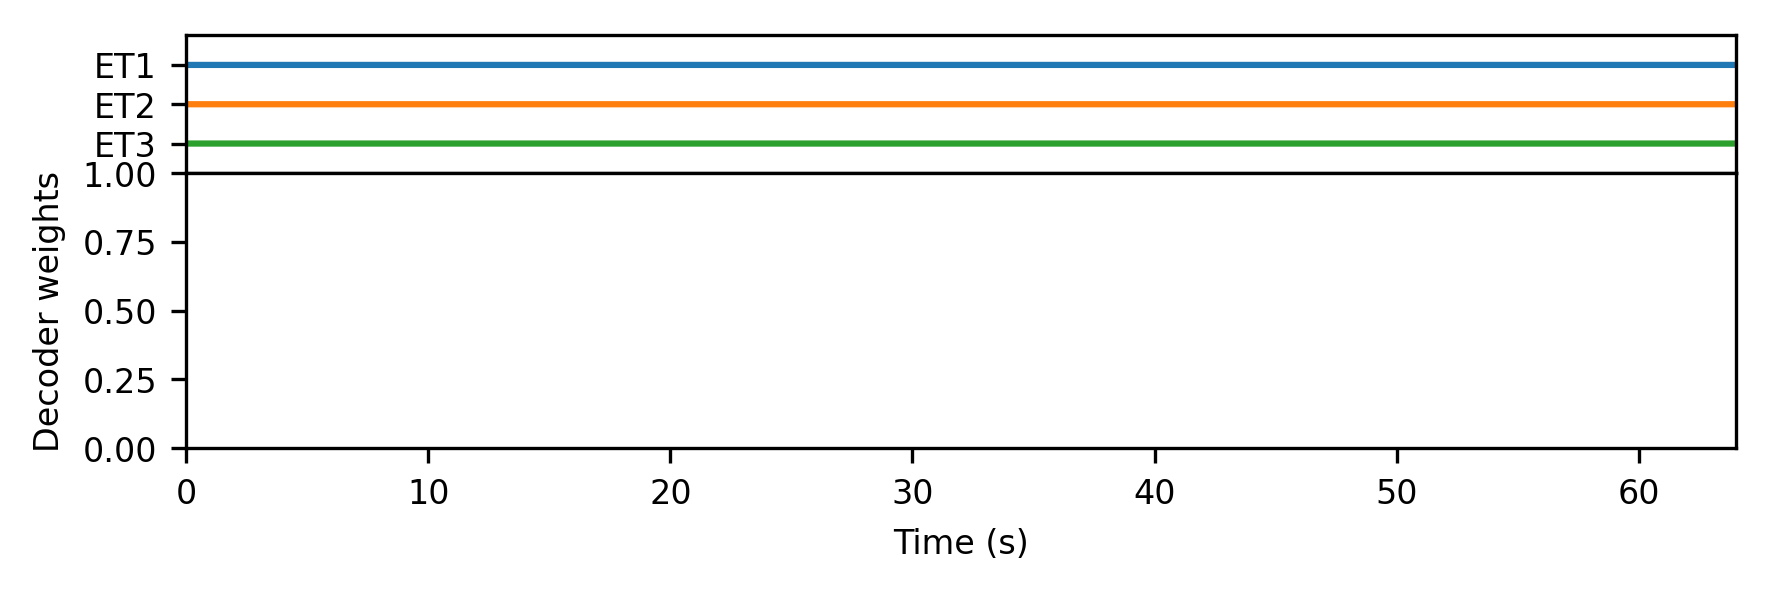
\includegraphics[
	width=15cm,
	trim=0 1cm 0 0,
	clip
	]{multiple_signal_detection/plots/out/300/detr/11}
	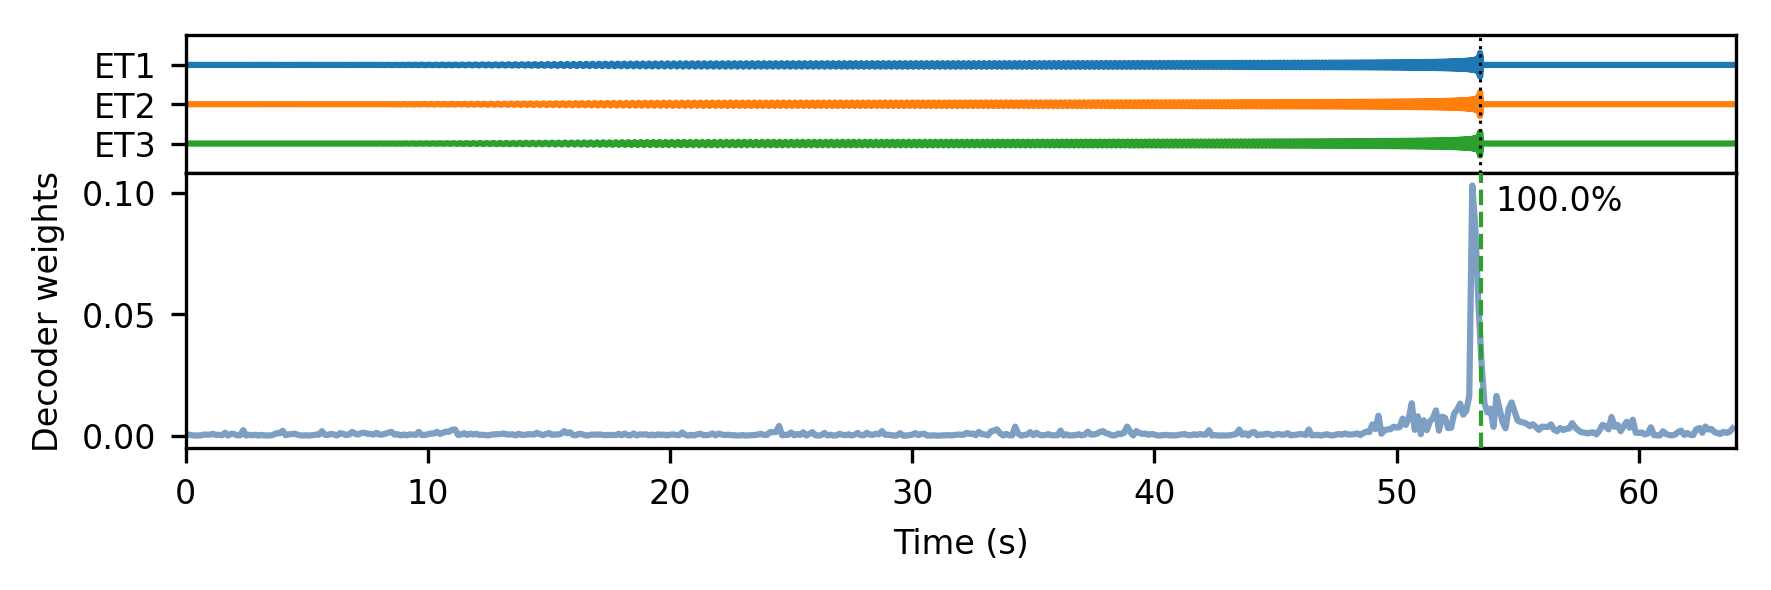
\includegraphics[
	width=15cm,
	trim=0 1cm 0 0,
	clip
	]{multiple_signal_detection/plots/out/300/detr/1}
	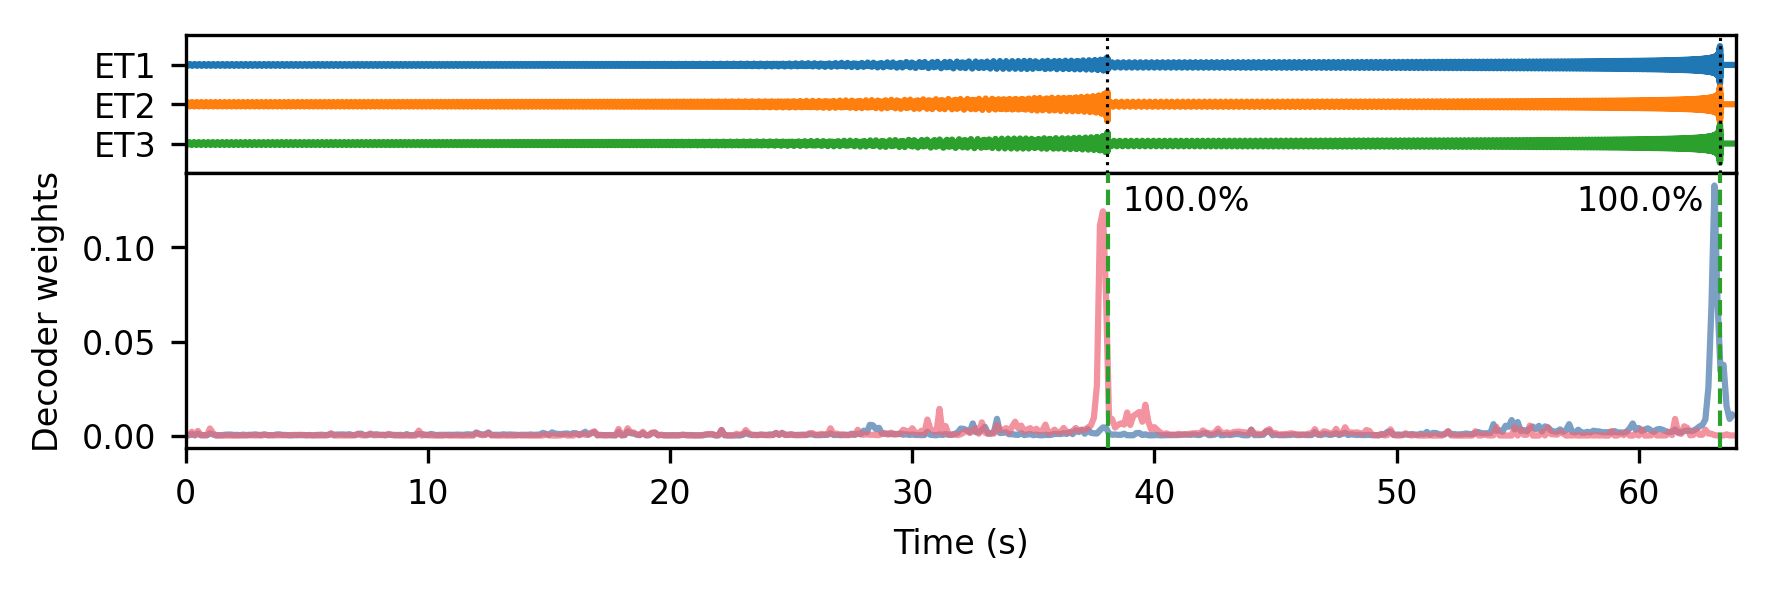
\includegraphics[
	width=15cm,
	trim=0 1cm 0 0,
	clip
	]{multiple_signal_detection/plots/out/300/detr/3}
	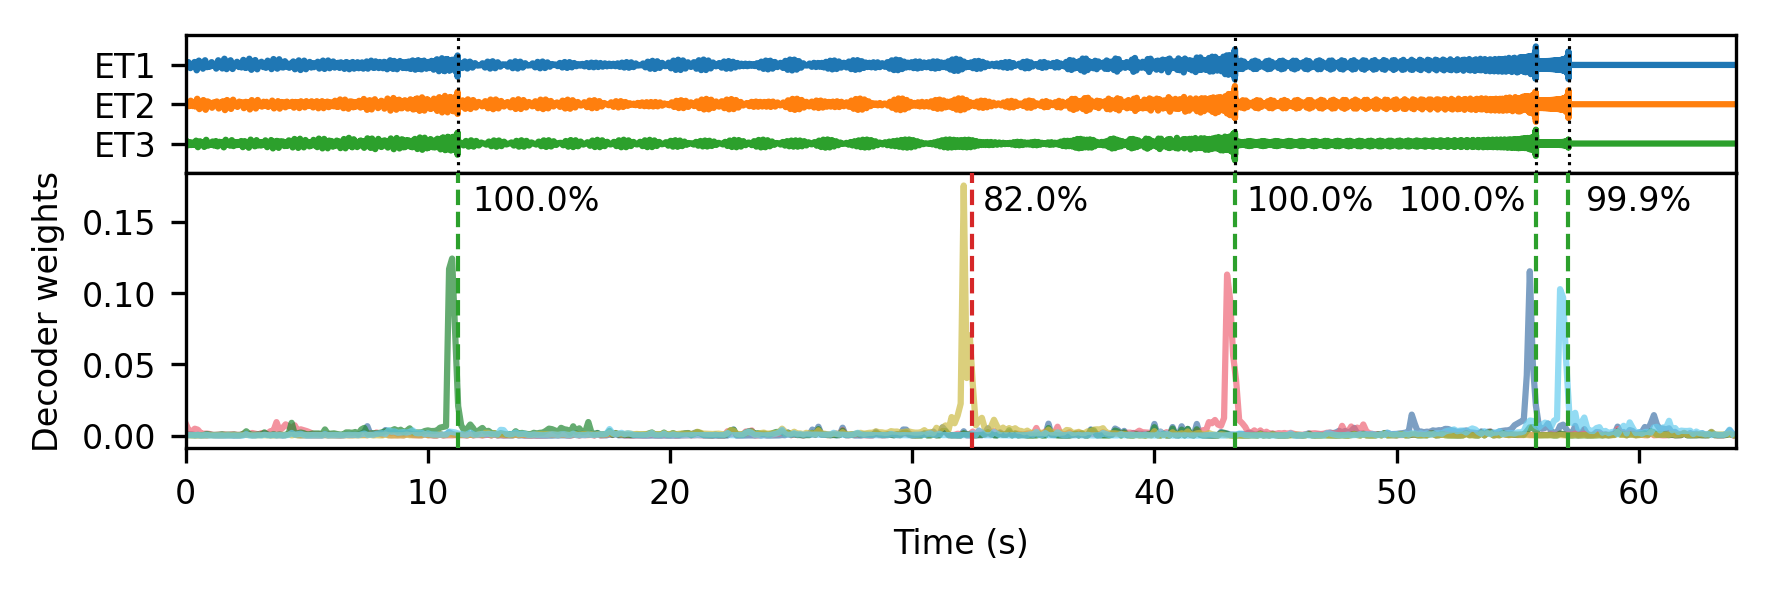
\includegraphics[
	width=15cm,
	trim=0 1cm 0 0,
	clip
	]{multiple_signal_detection/plots/out/300/detr/0}
	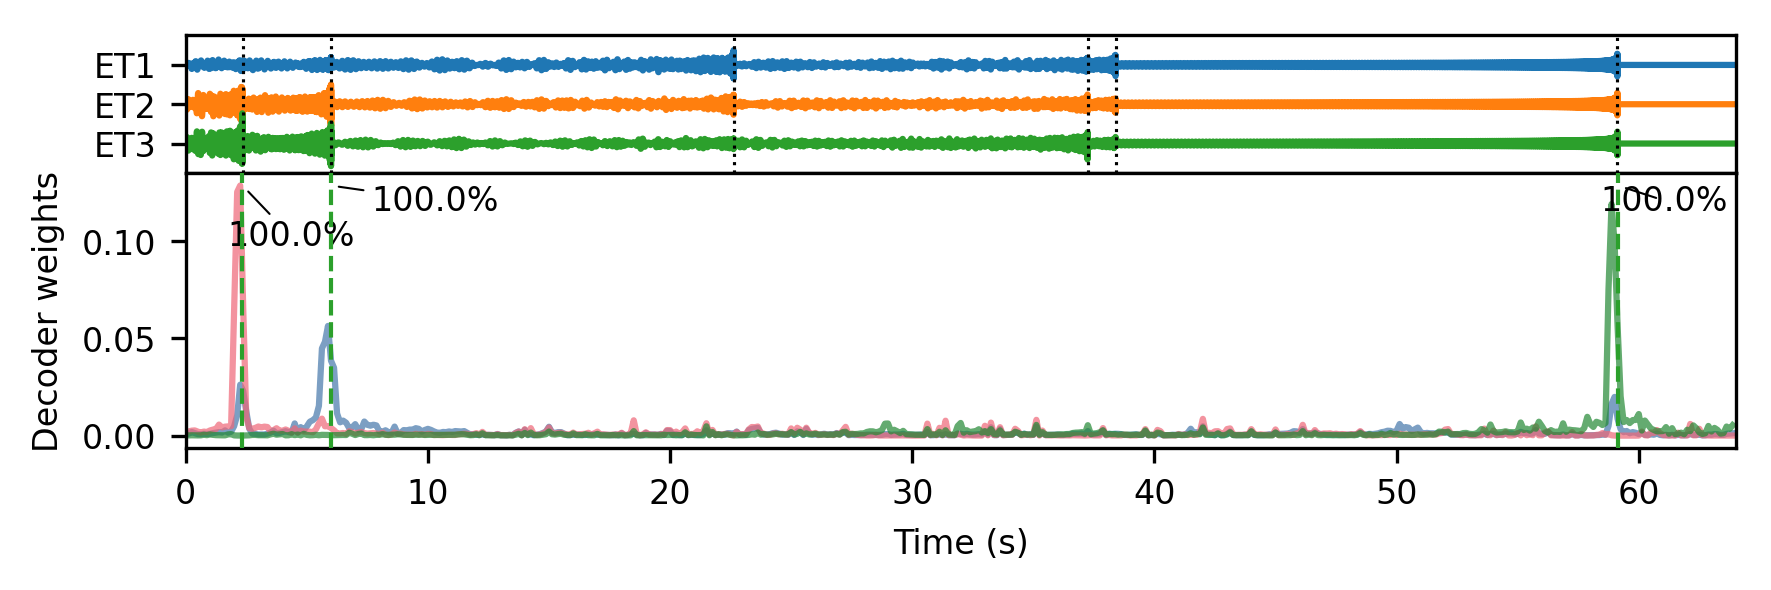
\includegraphics[
	width=15cm,
	]{multiple_signal_detection/plots/out/300/detr/8}
	\caption{DETR output for five samples. Each query is a GW candidate. These are plotted in the same manner as in Fig.~\ref{fig:heatmap:encoder_out}, and only candidates with scores exceeding \SI{69}{\percent} are shown. For each prediction, query--time cross-attention is plotted in different colors.}
	\label{fig:detr:out}
\end{figure}

% look at examples
% queries produce meaningful gw candidates
% choosing a threshold of 69%, FPs are rather low, while GW can be retrieved
% queries attend to time series through cross attention
% each query focuses on one signal

The following results and discussion largely mirror the structure of the previous chapter. The DETR model is evaluated on the same \SI{131}{\kilo\nothing}-sample test dataset, and GW candidates are assigned to signals with greedy matching. See the methodology in  Ch.~\ref{sec:heatmap:setup}.

It is again insightful to first inspect individual model outputs. See five examples in Fig.~\ref{fig:detr:out}. It can be seen that the DETR queries produce meaningful GW candidates. By applying a class-score threshold of \SI{69}{\percent}, most signals can be retrieved while keeping the number of FPs small. The choice of this threshold is justified later on. The predicted coalescence times also appear sufficiently accurate for the matching criterion $|t-\hat{t}|\leq\SI{0.1}{\second}$ used in this work.

The DETR prediction queries can attend to the time series through cross-attention.
The plots in Fig.~\ref{fig:detr:out} indicate that each query focuses mostly on a localized region of the input, close to the corresponding signal coalescence time.

\begin{figure}
	\centering
	\makebox[\textwidth]{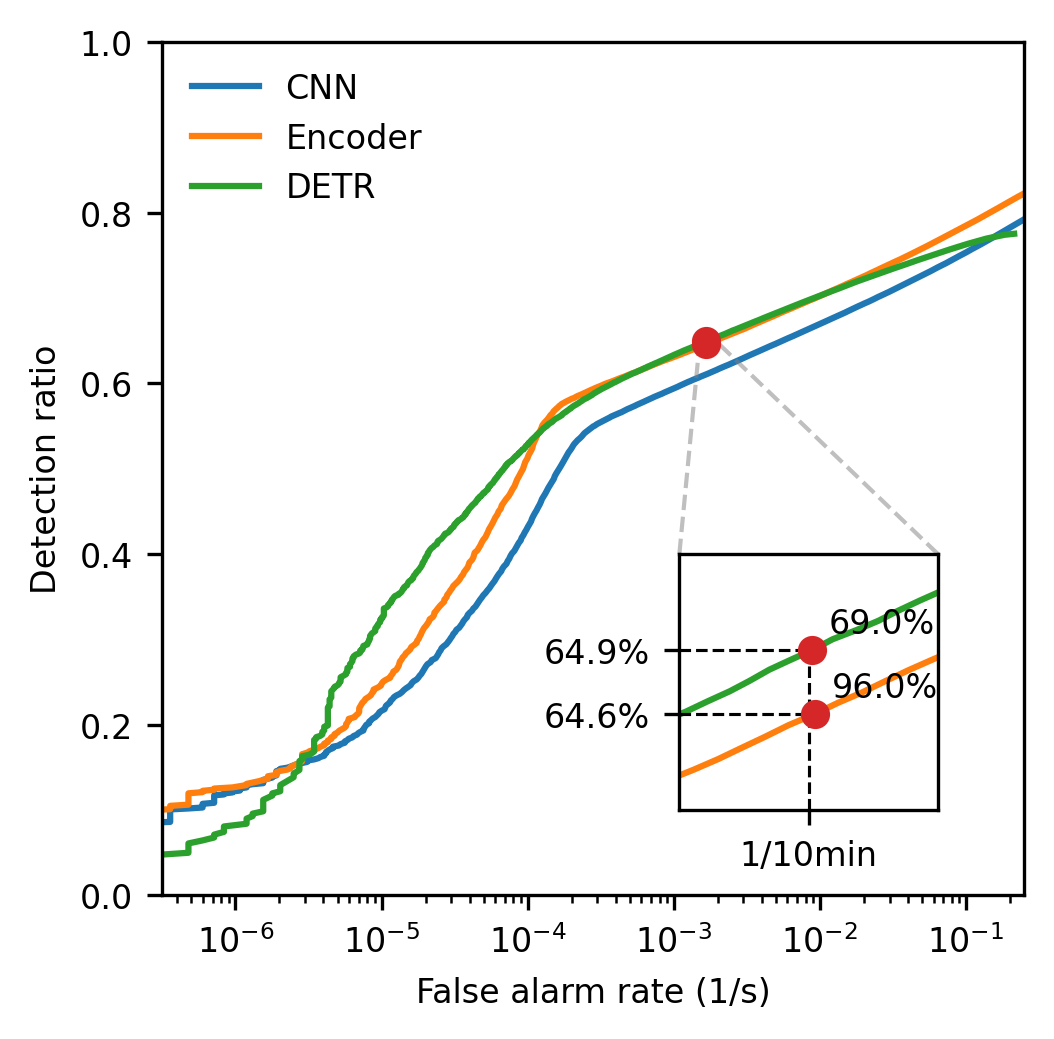
\includegraphics[width=9cm]{multiple_signal_detection/plots/cnn_encoder_detr_far}}
	\caption{Detection ratio as a function of FAR for the CNN heatmap regressor (\emph{blue}), transformer-encoder heatmap regressor (\emph{orange}), and DETR model (\emph{green}).}
	\label{fig:detr:far}
\end{figure}

% Performance comparison -> detection ratio against FAR
% see fig
% for high fars very similar to encoder
% for 10^-4<far<10^-5 -- 10^-6 better
% for really low far worse than both heatmap regressors
% comparable or even better performance that Encoder heatmap regressors while removing the need for postprocessing
% for low far performance maybe finetune with greedy matching

A quantitative comparison is obtained by varying the score threshold and computing the detection ratio and FAR over the full test dataset. Figure~\ref{fig:detr:far} compares the resulting operating characteristic of DETR with both heatmap regressors from the previous chapter. Over a large part of the FAR range, DETR performs comparably to the transformer heatmap model. For FARs from $\approx\SI{E-4}{\per\second}$ down to values between $\SI{E-5}{\per\second}$ and $\SI{E-6}{\per\second}$, DETR even reaches a higher detection ratio. At the lowest FARs, however, DETR falls below both heatmap regressors.

% TODO: DETR value was guessed in the 2nd nachkommastelle
At the fixed FAR operating point of $1/\SI{10}{\minute}$, DETR reaches a similar detection ratio of \SI{64.90(8)}{\percent}, compared to \SI{64.61(8)}{\percent} for the transformer-encoder heatmap regressor. The corresponding score threshold is \SI{69.0}{\percent}. Thus, DETR achieves comparable performance to heatmap regression while directly producing candidate scores and times, without requiring any post-processing steps.

\begin{figure}
	\centering
	\makebox[\textwidth]{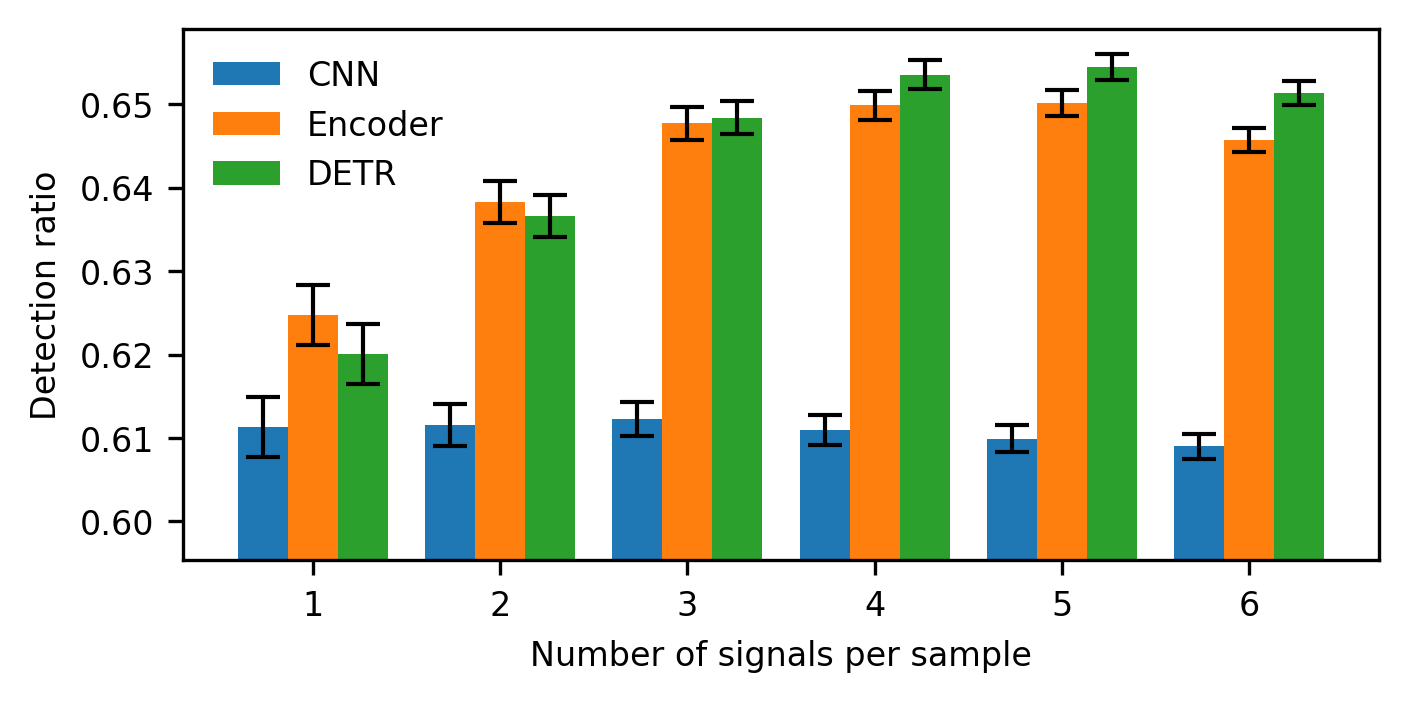
\includegraphics[width=12cm]{multiple_signal_detection/plots/cnn_encoder_detr_mergers}}
	\caption{Detection ratio as a function of the number of mergers per sample $n$. CNN heatmap regressor (\emph{blue}), transformer-encoder heatmap regressor (\emph{orange}), and DETR model (\emph{green}).}
	\label{fig:detr:num_mergers}
\end{figure}

% by looking at the performance with the number of mergers the same performance increase for samples with many signals can be observed
% because its also a transformer network and can exploit global information

The dependence on the number of signals per sample is shown in Fig.~\ref{fig:detr:num_mergers}. For $n=1$, DETR reaches comparable performance to the other models. Similar to the transformer-encoder heatmap regressor, DETR improves for larger $n$ as the detection ratio increases by \SI{3.4(4)}{\percent}.
This is consistent with DETR's use of global attention, which already appeared advantageous in the transformer heatmap regressor.

\begin{figure}
	\centering
	\makebox[\textwidth][c]{
		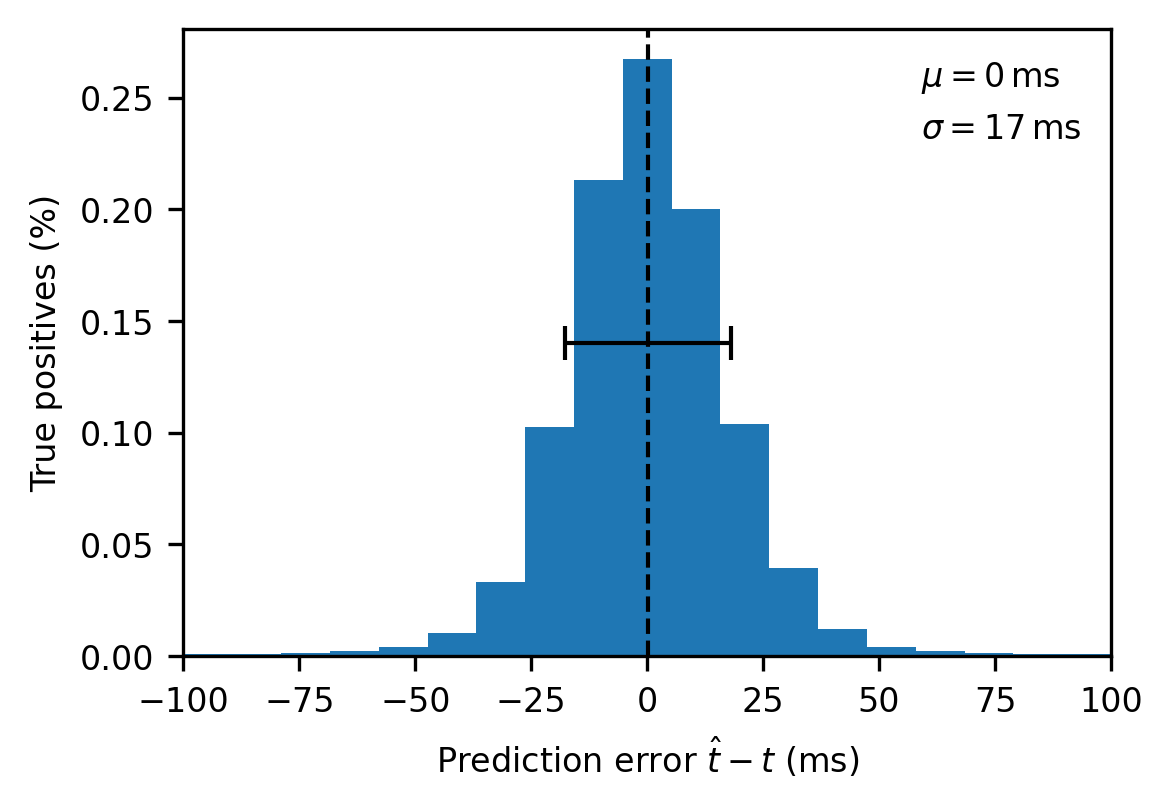
\includegraphics[width=8cm]{multiple_signal_detection/plots/detr_time}
		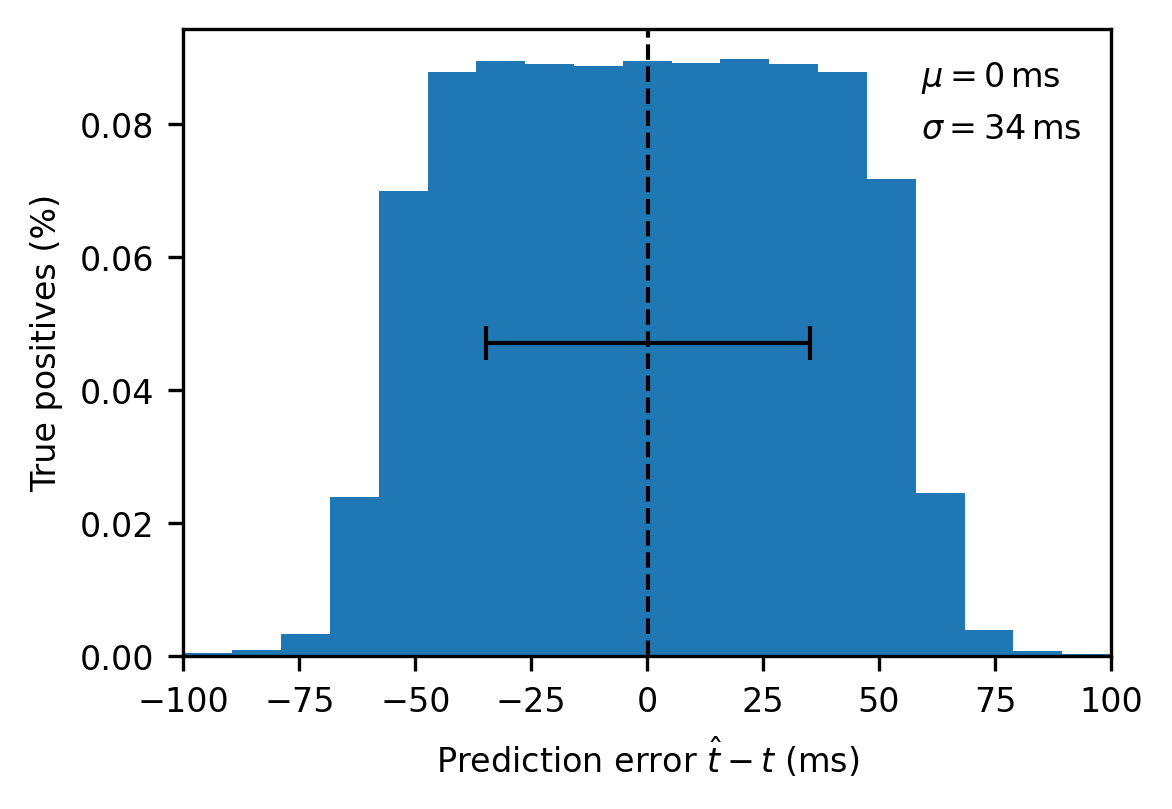
\includegraphics[width=8cm]{multiple_signal_detection/plots/encoder_time}
	}
	\caption{Prediction time error $\hat{t}-t$ for DETR (\emph{left}) and the transformer heatmap-regressor (\emph{right}). A vertical line shows the distribution mean $\mu$ and an error bar the standard deviation $\sigma$. The x-axis limits correspond to the matching criterion $|t-\hat{t}|\leq\SI{0.1}{\second}$.}
	\label{fig:detr:encoder_detr_time_acc}
\end{figure}

An important difference between DETR and heatmap regression is the way coalescence times are predicted. In heatmap regression, predictions are obtained by peak extraction and a local soft-argmax, while DETR predicts coalescence times directly. The effect on prediction time-accuracy is investigated by computing the error $\hat t - t$ for all TP predictions. 
The errors are plotted as histograms for both models in Fig.~\ref{fig:detr:encoder_detr_time_acc}.

% look at time prediction accuracy
% much better than encoder heatmap
% compute mean and std

Both error distributions have zero mean. For DETR, the distribution is sharper with a standard deviation of \SI{17}{\milli\second} compared to \SI{34}{\milli\second} for the heatmap regressor. Thus, DETR improves the time-prediction accuracy.

\section{Injection Study}

% no limitation because of heatmap resolution and better time accuracy -> probably better at close mergers

The previous chapter showed that heatmap regression becomes limited for nearby signals with $\Delta t_\text{coa}\leq\SI{0.3}{\second}$, as the two heatmap peaks can no longer be distinguished. Since DETR predicts coalescence times directly, one might expect improved performance for close overlaps. To test this, the same two-signal injection study as in the previous chapter is repeated for DETR.

\begin{figure}
	\centering
	\makebox[\textwidth]{
		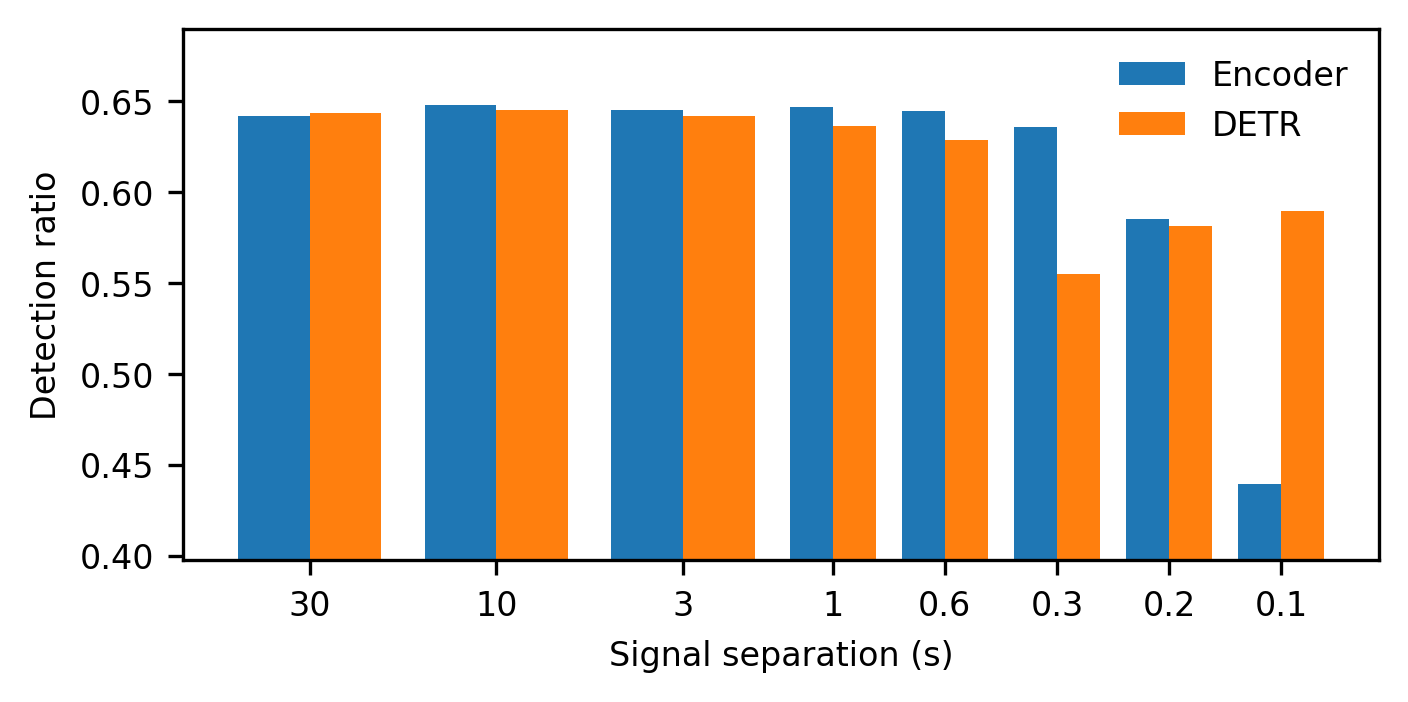
\includegraphics[width=12cm]{multiple_signal_detection/plots/encoder_detr_deltat}
	}
	\caption{Detection ratio as a function of signal separation for the transformer-encoder heatmap regressor (\emph{blue}) and for DETR (\emph{orange}). Computed over \SI{66}{\kilo\nothing} samples with \SI{131}{\kilo\nothing} signals. Uncertainties are too small to be visualized.}
	\label{fig:detr:detr_deltat}
\end{figure}

% do the same plot as before (see fig)
% network retains performance although it seems to be less robust than heatmap
% intermediate regime: worse?
% close regime: better because not limited

Fig.~\ref{fig:detr:detr_deltat} shows the detection ratio as a function of coalescence-time separation. The plot shows that, for separations $\geq\SI{3}{\second}$, both models perform equally well. DETR exhibits a performance decrease for separations of $\leq\SI{1}{\second}$ compared to $\leq\SI{0.3}{\second}$ for the heatmap regressor. However, this decrease is less pronounced for close separations of $\SI{0.1}{\second}$, where DETR retains a detection ratio of \SI{59.0(1)}{\percent} compared to \SI{43.9(1)}{\percent}. 

% look at delta t cases
% can predict multiple signals regardless of dt
% it does seem to struggle identifying signals if they are close
% especially in the strong regime dt<1s
% detr not perfect for close overlaps but is at least not limited in resolution in principle (we can also see this by look at these plots)

A more detailed view is obtained by distinguishing the four recovery cases: only the earlier signal A is recovered, only the later signal B, both signals are recovered, or both signals are missed. The result is shown in Fig.~\ref{fig:detr:deltat_cases}, together with the corresponding heatmap-regression result. Three example outputs are shown in Fig.~\ref{fig:detr:deltat_plot} as well. 

DETR can still output two GW candidates for separations of $\leq\SI{1}{\second}$, but the fraction of samples where both signals are recovered decreases in the close-overlap regime. Instead, single-signal recoveries become more common. This suggests that, while DETR \emph{can} make predictions regardless of signal coalescence-time separation, it is not perfectly robust when disentangling close overlaps. 

\begin{figure}
	\centering
	\makebox[\textwidth]{
	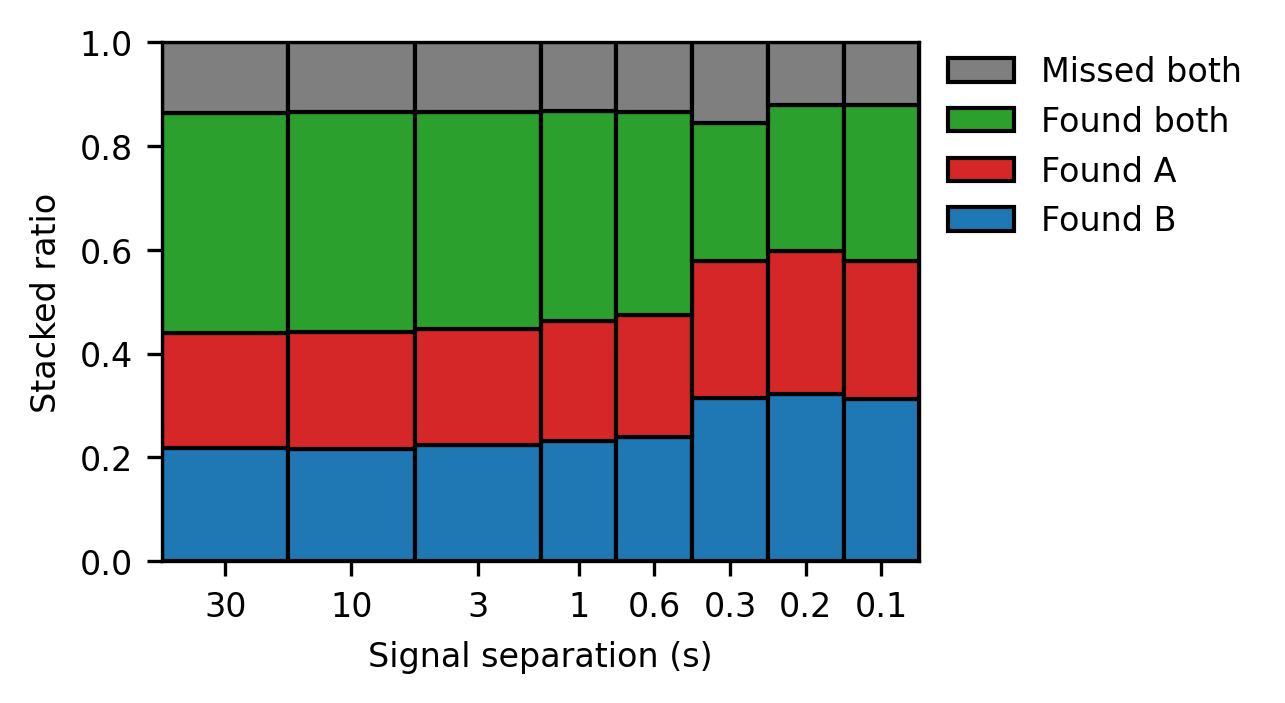
\includegraphics[
	height=6cm, 
	trim=0 0 3cm 0,
	clip]{multiple_signal_detection/plots/detr_stacked}
	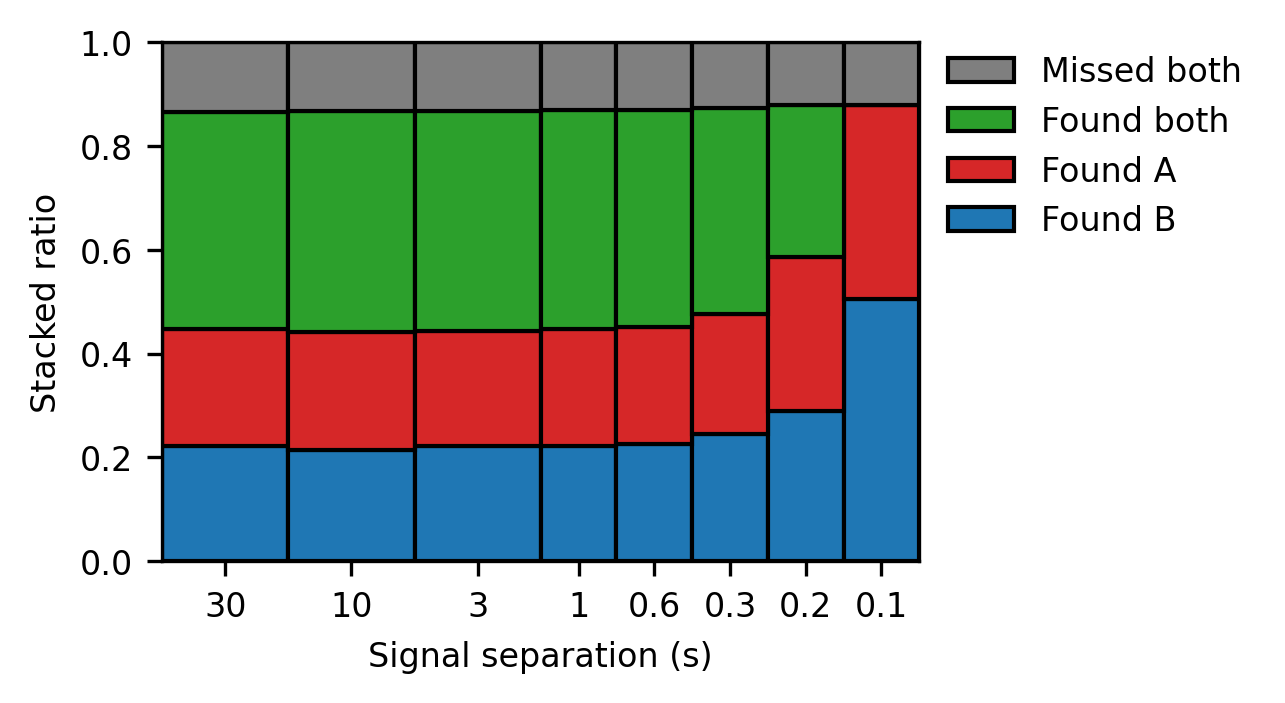
\includegraphics[
	height=6cm, 
	trim=1.3cm 0 0 0,
	clip]{multiple_signal_detection/plots/encoder_stacked}
	}
	\caption{Performance with signal separation for DETR (\emph{left}) and for the heatmap regressor (\emph{right}).}
	\label{fig:detr:deltat_cases}
\end{figure}

\begin{figure}
	\centering
	\makebox[\textwidth]{
		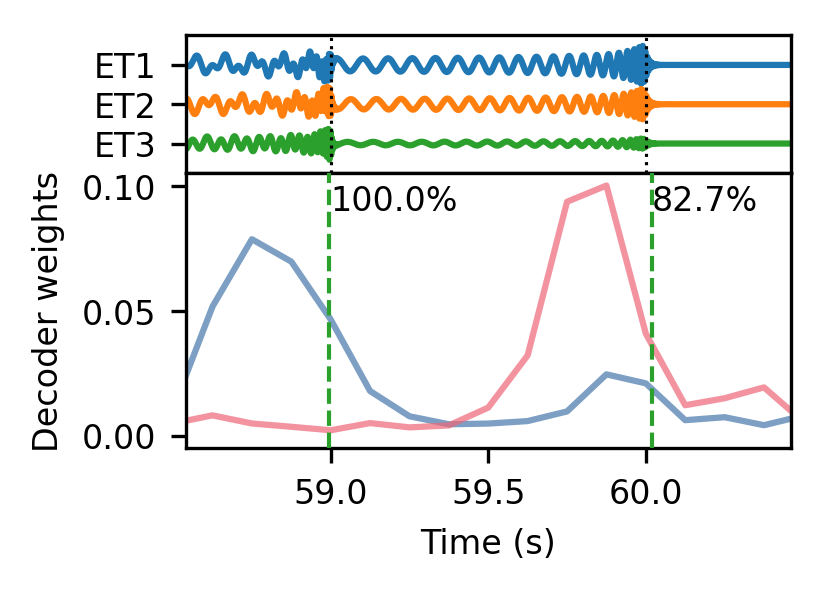
\includegraphics[
		height=5cm,
		trim=0 0 0 0,
		clip
		]{multiple_signal_detection/plots/out/700/detr/0_zoom}
		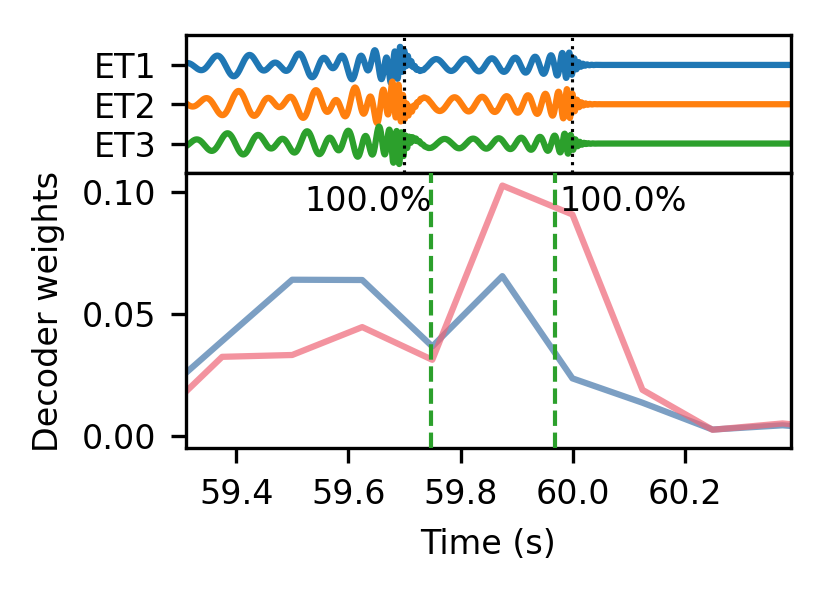
\includegraphics[
		height=5cm,
		trim=1.35cm 0 0 0,
		clip
		]{multiple_signal_detection/plots/out/800/detr/7_zoom}
		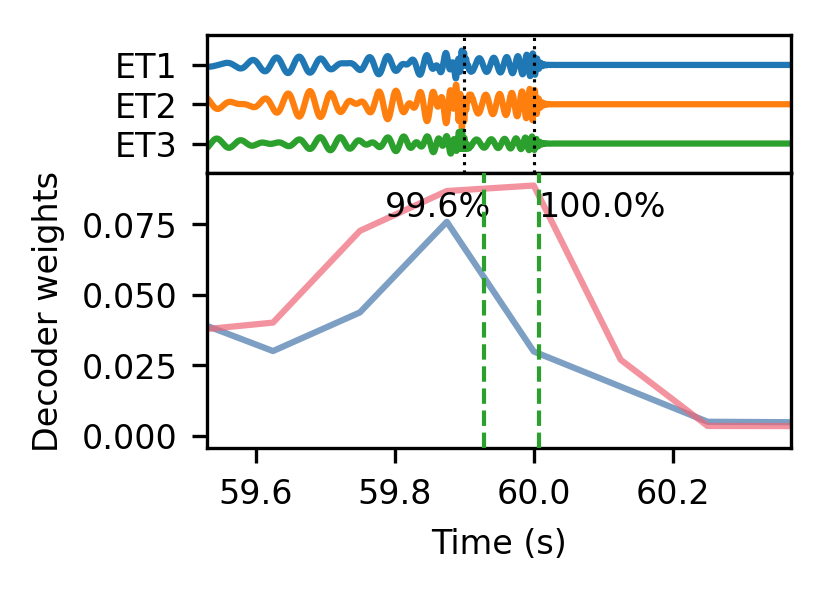
\includegraphics[
		height=5cm,
		trim=1.5cm 0 0 0,
		clip
		]{multiple_signal_detection/plots/out/900/detr/6_zoom}
	}
	\caption{Three example DETR outputs for $\Delta t_\text{coa}=\SI{1}{\second}$ (\emph{left}), $\Delta t_\text{coa}=\SI{0.3}{\second}$ (\emph{middle}) and $\Delta t_\text{coa}=\SI{0.1}{\second}$ (\emph{right}).}
	\label{fig:detr:deltat_plot}
\end{figure}

\section{Discussion}

% DETR performs comparably well
% removes intrinsic bottleneck of heatmap resolution
% easily adapted to produce parameter estimates as well
% direct time prediction yields better results (in a way this is promising for parameter estimation)

DETR demonstrates performance comparable to the heatmap transformer while eliminating its intrinsic bottleneck, the heatmap time-resolution. By directly predicting coalescence times, DETR achieves improved time-accuracy. DETR is easily adapted to predict additional signal parameters in future work.

% Performance still degrades in the edge cases of low fars and close signal separations
% may be attributed to the larger model size and insufficient training (refer to learning curves)

Despite these advantages, the model exhibits reduced performance for low FARs and moderately separated signals with $\SI{1}{\second}\geq\Delta t_\text{coa}\geq\SI{0.3}{\second}$. 
In the regime $\Delta t_\text{coa}\leq\SI{0.2}{\second}$, performance is comparable to or exceeds that of the heatmap regressor, as DETR is free to predict GW candidates regardless of signal separation.

One possible explanation is that these limitations arise from insufficient model optimization rather than architectural flaws. DETR comprises \SI{6.2}{\mega\nothing} trainable parameters compared to roughly \SI{2.2}{\mega\nothing} for the heatmap transformer, while being trained on the same \SI{1}{\mega\nothing} sample dataset. The learning curves (Figs.~\ref{fig:detr:learning_curve} and \ref{fig:detr:tandem}) show that DETR continues improving until epoch $93$, considerably later than the heatmap transformer, which overfit at the 16th epoch. This behavior suggests that additional training and larger datasets might further improve performance.

% future: maybe finetune on the same matching that is used for evaluation instead of hungarian (which is less robust for low fars and clos separations)

Another potential direction is to better align the matching algorithm DETR uses for training (Hungarian matching) with the one employed for evaluation (greedy matching). It can be argued that greedy matching is more robust in low-FAR operating regimes, where DETR has shown worse performance compared to heatmap regression. This is because at low FARs, greedy matching neglects all predictions with scores $\lesssim\SI{100}{\percent}$ and assigns only the highest-score predictions. In contrast, Hungarian matching considers \emph{all} predictions for assignment by minimization of some cost function instead. 
In future work, a one-to-one matching algorithm that is more robust at low FARs like greedy matching could be used for fine-tuning DETR for improved performance in this operating regime.